\section{Results}

All the following benchmarks were conducted on a GitHub-hosted virtual machine
under GitHub Actions, running Ubuntu 24.04.2 LTS (Noble Numbat) with an AMD
EPYC 7763 64-Core Processor (x86\_64 architecture) operating at 3.24 GHz,
configured with 2 CPU cores and 2 threads per core, and 7.8GB of available RAM.
The system utilizes a 75GB SSD with ext4 filesystem, achieving 1.5 GB/s write
throughput in basic I/O tests. Network connectivity is provided through a 1500
MTU Ethernet interface. All tests were conducted on OpenJDK 21 (Correto build)
with the G1 garbage collector enabled by default. The following . JVM arguments
were used: \texttt{-Xms512m -Xmx16g}. Each test was executed 5 times per
configuration to ensure the reliability of the results.

All template engines were configured to use UTF-8 encoding and disable
automatic HTML escaping to ensure fair comparison and consistent output across
all template engines. Caching behaviour was left as the default for each
engine, allowing them to optimize template loading and rendering as per their
design. These configurations ensure that all engines operate under equivalent
conditions, with template loading, encoding, and escaping behavior normalized
across implementations.

For both the Apache Bench and JMeter tests, we simulate a 1000-request warmup
period for each route with a concurrent user load of 32 users. The warmup
period is followed by the actual test period, during which we simulate 256
requests per user, scaling in increments up to 128 concurrent users.

The results are presented in the form of throughput (number of requests per
second) for each template engine, with the x-axis representing the number of
concurrent users and the y-axis representing the throughput in requests per
second.

Both Quarkus and Spring MVC implementations were configured with an 8KB output
buffer size to ensure consistency, despite Quarkus not enabling PSSR at this
size and Spring MVC not supporting PSSR for the tested templates. Testing with
a reduced 512B buffer size showed only a 0.046\% performance difference with
Rocker, indicating negligible impact. Both frameworks use unlimited platform
thread pools, enabling on-demand thread creation up to system limits for
maximum throughput and scalability observation under high concurrent load.

Since the obtained results for JMeter and Apache Bench show no significant
differences, only the JMeter results will be presented. Statistical analysis of
test configurations revealed an average absolute percentage difference of
2.83\% between the two load testing tools. While individual approach
differences ranged from -16.53\% to +14.66\% at the extremes, the consistent
directional bias and small magnitude of differences indicate that both tools
provide comparable performance measurements. Given this statistical equivalence
and the need for brevity, only JMeter results are presented, as they provide
representative performance characteristics across all tested configurations.

\subsection{Scalability results for the \texttt{Presentations} class}

The results in Figure~\ref{fig:presentations-webflux-jmeter} depict the
throughput (number of requests per second) for each template engine, with
concurrent users ranging from 1 to 128, from left to right. The benchmarks
include HtmlFlow using suspendable web templates (\textit{HtmlFlow-Susp},
equivalent to the approach shown in Listing~\ref{lst:presentation-flow}),
Jstachio using Virtual Threads with the \texttt{Iterable} interface
(\textit{Jstachio-Virtual}), and Thymeleaf using the reactive View Resolver
driver (Thymeleaf-Rx). \textit{Blocking} and \textit{Virtual} represent the
average throughput of the blocking approaches (i.e., KotlinX, Rocker, Jstachio,
Pebble, Freemarker, Trimou, HtmlFlow, and Thymeleaf) when run in the context of
a separate coroutine dispatcher or Virtual Threads, respectively.

We show the \textit{HtmlFlow-Susp}, \textit{Jstachio-Virtual}, and
\textit{Thymeleaf-Rx} engines separately to observe the performance of the
non-blocking engines when using the Suspending, Virtual Thread, and Reactive
approaches. The \textit{Blocking} and \textit{Virtual} are aggregated due to
the similar performance of different engines when using those approaches.

\begin{figure}[h]
     \centering
     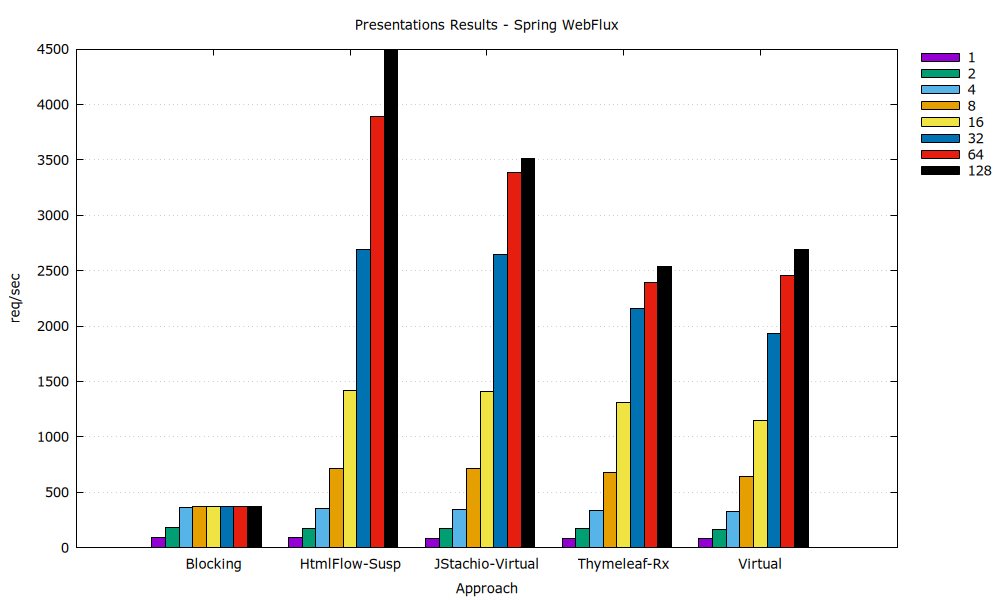
\includegraphics[width=0.8\textwidth]{./Graphs/presentations-webflux-jmeter.png}
     \caption{Throughput (requests per second) scalability results for Spring Webflux with \texttt{Presentations} class}\label{fig:presentations-webflux-jmeter}
\end{figure}

The results in Figure~\ref{fig:presentations-webflux-jmeter} show that when
using blocking template engines with a separate coroutine dispatcher, the
engines are unable to scale effectively beyond 4 concurrent users. In contrast,
\textit{HtmlFlow-Susp} scales up to 128 concurrent users, achieving 4,487
requests per second. When blocking approaches are executed in the context of
Virtual Threads—thus enabling non-blocking I/O—the engines scale up to 64
concurrent users, with Jstachio using Virtual Threads reaching 3,514 requests
per second. The Thymeleaf implementation using the reactive View Resolver
driver scales up to 32 concurrent users, achieving a lower maximum throughput
of 2,559 requests per second.

It is important to note that the differences in scalability and throughput
between the \textit{HtmlFlow-Susp}, \textit{Jstachio-Virtual}, and
\textit{Thymeleaf-Rx} approaches may be influenced by the specific template
engines used, rather than the approach itself. When comparing the
\textit{Reactive}, \textit{Suspendable}, and \textit{Virtual} approaches
specifically with HtmlFlow, we found that all three achieve similar
performance: HtmlFlow using a blocking approach with Virtual Threads reaches
4,691 requests per second, while HtmlFlow using a reactive approach achieves
4,792 requests per second.

\begin{figure}[h]
     \centering
     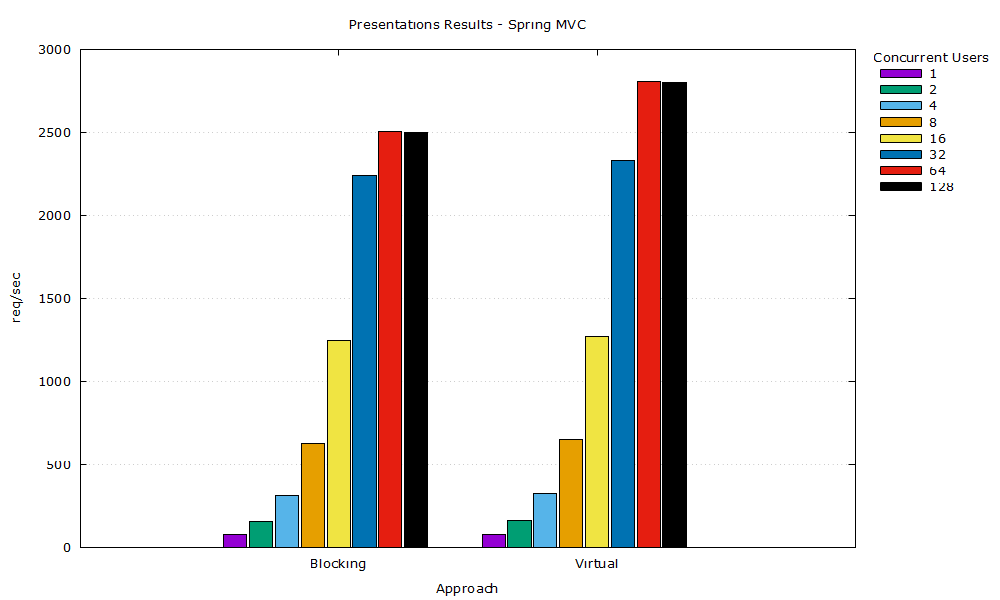
\includegraphics[width=0.8\textwidth]{./Graphs/presentations-springmvc-jmeter.png}
     \caption{Throughput (requests per second) scalability results for Spring MVC with \texttt{Presentations} class}\label{fig:presentations-springmvc-jmeter}
\end{figure}

% The results for the Spring MVC implementation, shown in
% Figure~\ref{fig:presentations-springmvc-jmeter}, compare two approaches:
% \textit{Blocking}, which uses platform threads with \texttt{StreamingResponseBody},
% and \textit{Virtual}, which uses Virtual Threads. Both approaches scale
% effectively up to 128 concurrent users, with the Virtual Thread approach
% achieving a slightly higher throughput of 9,000 requests per second. However,
% these values are slightly lower than those observed in the Spring WebFlux
% implementation.
The results for the Spring MVC implementation, shown in
Figure~\ref{fig:presentations-springmvc-jmeter}, compare two synchronous
approaches: \textit{Blocking}, which uses platform threads with
\texttt{StreamingResponseBody}, and \textit{Virtual}, which uses Virtual
Threads. Since Spring MVC follows a thread-per-request architecture, the
asynchronous approaches—\textbf{Reactive} and \textbf{Suspendable}—described in
Section~\ref{sec:bench} are not applicable. Both the \textit{Blocking} and
\textit{Virtual} strategies scale effectively up to 32 concurrent users, with
the Virtual Threads approach achieving a slightly higher maximum throughput of
2,797 requests per second, compared to 2,498 requests per second for the
blocking approach. These results indicate that while Spring MVC can handle a
moderate level of concurrency, it does not reach the scalability of the
reactive or suspendable approaches available in Spring WebFlux. Furthermore,
Spring MVC does not enable Progressive Server-Side Rendering (PSSR) for the
tested templates, as previously discussed in Section~\ref{sec:bench}.

\begin{figure}[h]
     \centering
     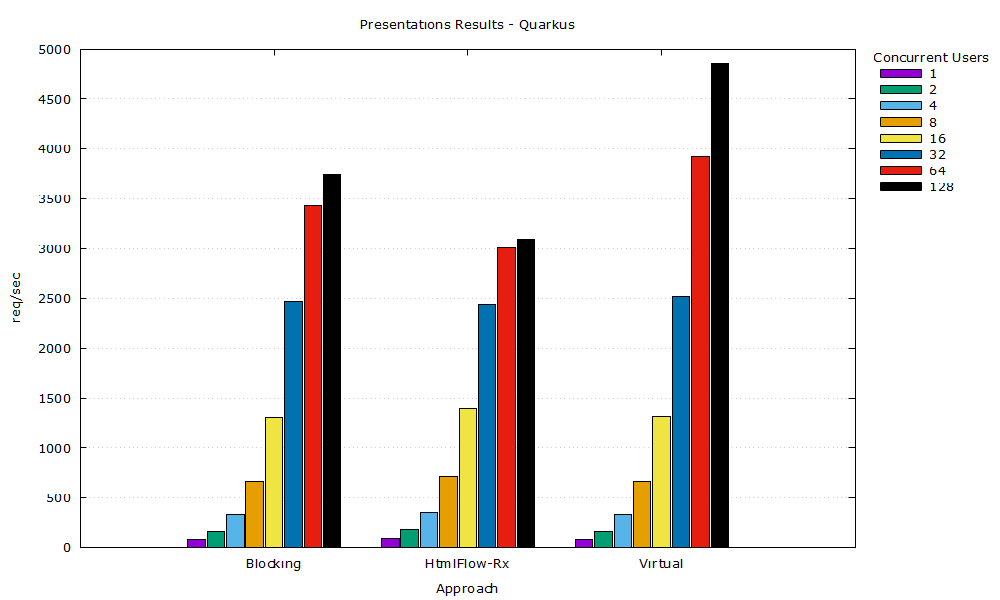
\includegraphics[width=0.8\textwidth]{./Graphs/presentations-quarkus-jmeter.png}
     \caption{Throughput (requests per second) scalability results for Quarkus with \texttt{Presentations} class}\label{fig:presentations-quarkus-jmeter}
\end{figure}

The results for the Quarkus implementation, shown in
Figure~\ref{fig:presentations-quarkus-jmeter}, indicate that Quarkus handles
synchronous approaches more efficiently than Spring WebFlux. The blocking
engines scale up to 64 concurrent users, achieving up to 3,744 requests per
second. When using Virtual Threads, the throughput increases even further,
reaching 4,856 requests per second, allowing scalability up to 128 users. This
demonstrates that Quarkus's implementation of Virtual Threads is effective for
enabling PSSR\@, and comparable to the \textit{Suspendable} and
\textit{Reactive} approaches used in Spring WebFlux in terms of scalability and
throughput.

Additionally, \textit{HtmlFlow-Rx}, a reactive implementation of the HtmlFlow
template engine (equivalent to the approach shown in
Listing~\ref{lst:presentation-observable}) that utilizes Quarkus's reactive
programming model, achieved a lower throughput than the the \textit{Blocking}
and \textit{Virtual} approaches—3,088 requests per second. This demonstrates
that Quarkus's reactive programming model is effective for enabling PSSR\@,
although it does not achieve the same level of performance or scalability as
the same approach in Spring WebFlux, stagnating after 32 concurrent users.

\subsection{Scalability results for the \texttt{Stocks} class}

\begin{figure}[h]
     \centering
     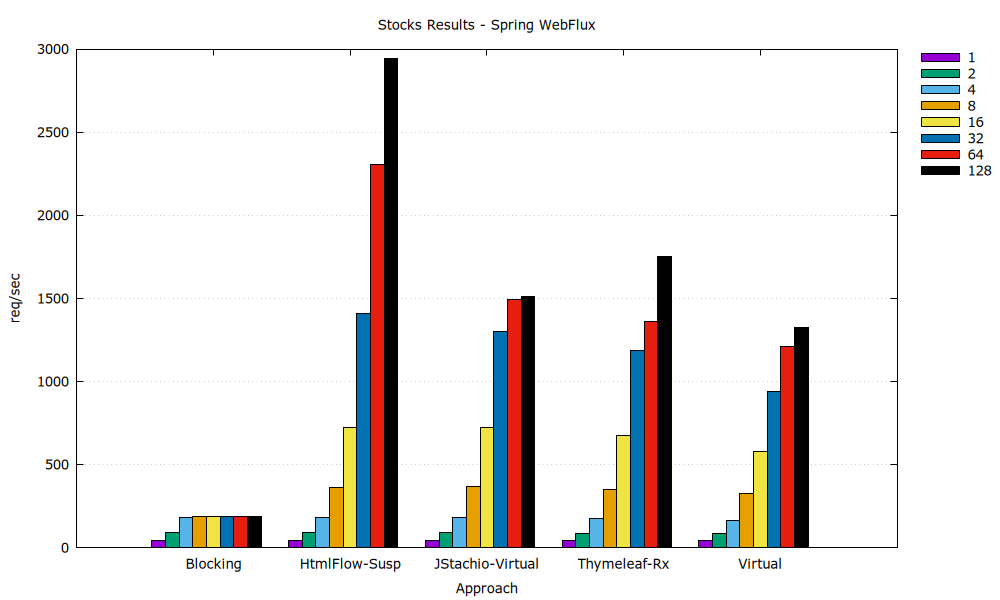
\includegraphics[width=0.8\textwidth]{./Graphs/stocks-webflux-jmeter.png}
     \caption{Throughput (requests per second) scalability results for Spring Webflux with \texttt{Stocks} class}\label{fig:stocks-webflux-jmeter}
\end{figure}

The results in Figure~\ref{fig:stocks-webflux-jmeter} use the same template
engines and approaches as the previous benchmark, but with a more complex data
model: the Stock class, which includes 20 instances and approximately two times
as many data bindings. With this data model, the scalability of the engines
remains largely unchanged; however, throughput is reduced across all engines.
Compared to the Presentation benchmark, Jstachio using virtual threads
experienced a more pronounced decrease in performance relative to the
\textit{Reactive} and \textit{Suspending} approaches, with Jstachio using
Virtual Threads now achieving 1,509 requests per second, compared to 1,750
requests per second achieved by the Thymeleaf implementation using the reactive
View Resolver driver.

It is again important to note that the differences in scalability and
throughput between the \textit{HtmlFlow-Susp}, \textit{Jstachio-Virtual}, and
\textit{Thymeleaf-Rx} approaches may be influenced by the specific template
engines used, rather than the approach itself. When comparing the
\textit{Reactive}, \textit{Suspendable}, and \textit{Virtual} approaches
specifically with HtmlFlow, we found that all three achieve similar
performance: HtmlFlow using a blocking approach with Virtual Threads reaches
3,090 requests per second, while HtmlFlow using a reactive approach achieves
3,026 requests per second. This indicates that the more pronounced decrease in
performance for Jstachio using Virtual Threads is likely due to the specific
implementation of the template engine, rather than the use of Virtual
Threads itself.

The overall throughput reduction across all engines is expected, as the Stock
class contains more data properties than the \texttt{Presentation} class,
adding overhead related to the data binding process of each template engine.

\begin{figure}[h]
     \centering
     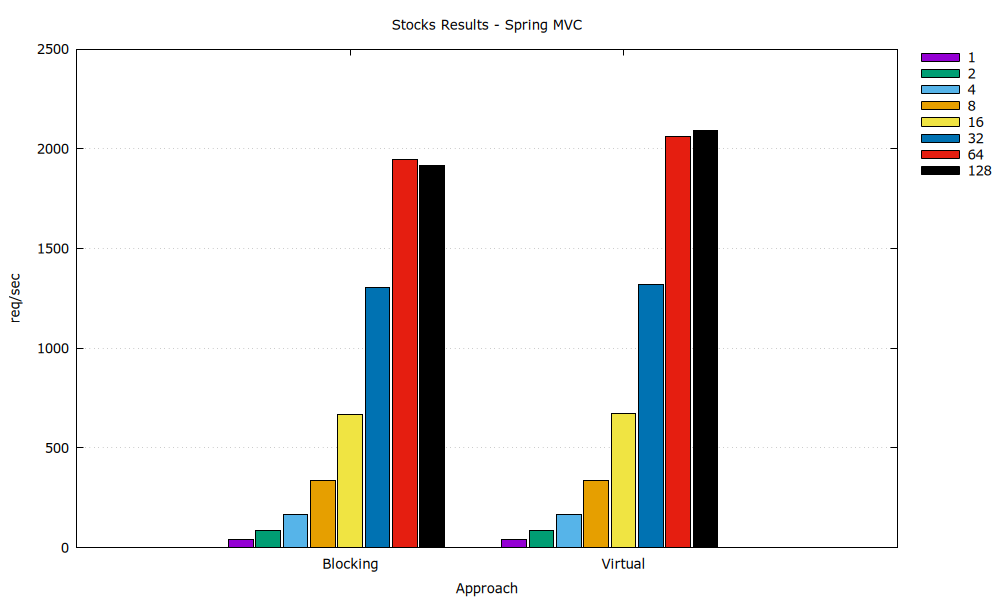
\includegraphics[width=0.8\textwidth]{./Graphs/stocks-springmvc-jmeter.png}
     \caption{Throughput (requests per second) scalability results for Spring MVC with \texttt{Stocks} class}\label{fig:stocks-springmvc-jmeter}
\end{figure}

The results shown in Figure~\ref{fig:stocks-springmvc-jmeter} indicate that the
Spring MVC implementation using the blocking approach with
\texttt{StreamingResponseBody} achieves a throughput of up to 1,916 requests
per second, with no significant improvement observed when using Virtual
Threads. Both approaches scale effectively up to 64 concurrent users. Although
these approaches achieve higher throughput in Spring MVC than in Spring
WebFlux, their overall performance remains lower than that of the reactive and
suspendable approaches.

\begin{figure}[h]
     \centering
     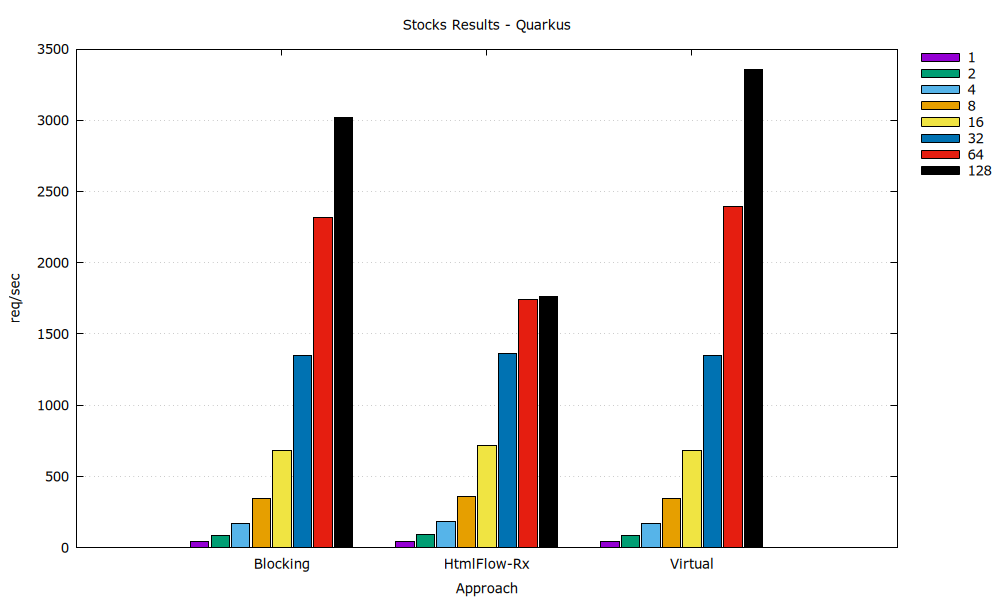
\includegraphics[width=0.8\textwidth]{./Graphs/stocks-quarkus-jmeter.png}
     \caption{Throughput (requests per second) scalability results for Quarkus with \texttt{Stocks} class}\label{fig:stocks-quarkus-jmeter}
\end{figure}

The results depicted in Figure~\ref{fig:stocks-quarkus-jmeter} show that the
Quarkus synchronous approaches scale effectively up to 128 concurrent users,
achieving performance comparable to the Spring WebFlux implementation. The
blocking approach reaches a throughput of 3,019 requests per second, while the
Virtual Threads approach achieves a throughput of 3,357 requests per second. In
addition to the synchronous engines, the \textit{HtmlFlow-Rx} approach also
achieves a throughput of 1760 requests per second, indicating that this
approach achieves lower performance in Quarkus than in Spring WebFlux, where it
reached 3,026 requests per second, as previously mentioned.

The results of the benchmarks show that non-blocking engines—whether using
reactive programming, Kotlin coroutines, or Java Virtual Threads—are able to
scale effectively, supporting between 32 and 128 concurrent users depending on
the approach and framework. Out of all the tested frameworks, Spring Webflux
showed itself the most effective at enabling PSSR, mostly due to its native
support for publish-subscribe interfaces, allowing for content to be streamed
as data becomes available, instead of when the response buffer is flushed.
Quarkus also enabled PSSR effectively, but it required additional configuration
of the \texttt{OutputBuffer} size to achieve the same results as Spring
Webflux. The Spring MVC implementation, on the other hand, did not enable PSSR
for the tested templates.

However, it is important to acknowledge the limitations of our chosen data
models for generalizability. The tested templates used relatively simple data
structures with limited nesting and straightforward property bindings.
Real-world applications often involve deeply nested data structures, complex
conditional logic, and iterative rendering over thousands of items. Under such
conditions, we anticipate significantly different performance characteristics:
increased memory consumption due to object traversal overhead, higher CPU
utilization for complex evaluations, and altered scalability patterns where
non-blocking approaches may become more advantageous. The performance
degradation observed with our Stock class benchmark—which merely doubled the
number of properties—suggests that enterprise-level template complexity would
result in substantially higher performance degradation. Future work should
investigate these scenarios with more realistic data models to better
understand performance boundaries and optimization strategies for complex PSSR
implementations.

\subsection{Memory Consumption and Resource Utilization Analysis}

This section evaluates the memory and CPU resource characteristics of three
representative concurrency models: Virtual Threads, suspendable coroutines, and
reactive streams. While previous benchmarks demonstrated that Virtual Threads
can offer comparable throughput to non-blocking paradigms, we now assess
whether this simplicity in code comes with higher runtime resource costs.

\textbf{Virtual Threads vs Suspendables}

\begin{figure}[h]
     \centering
     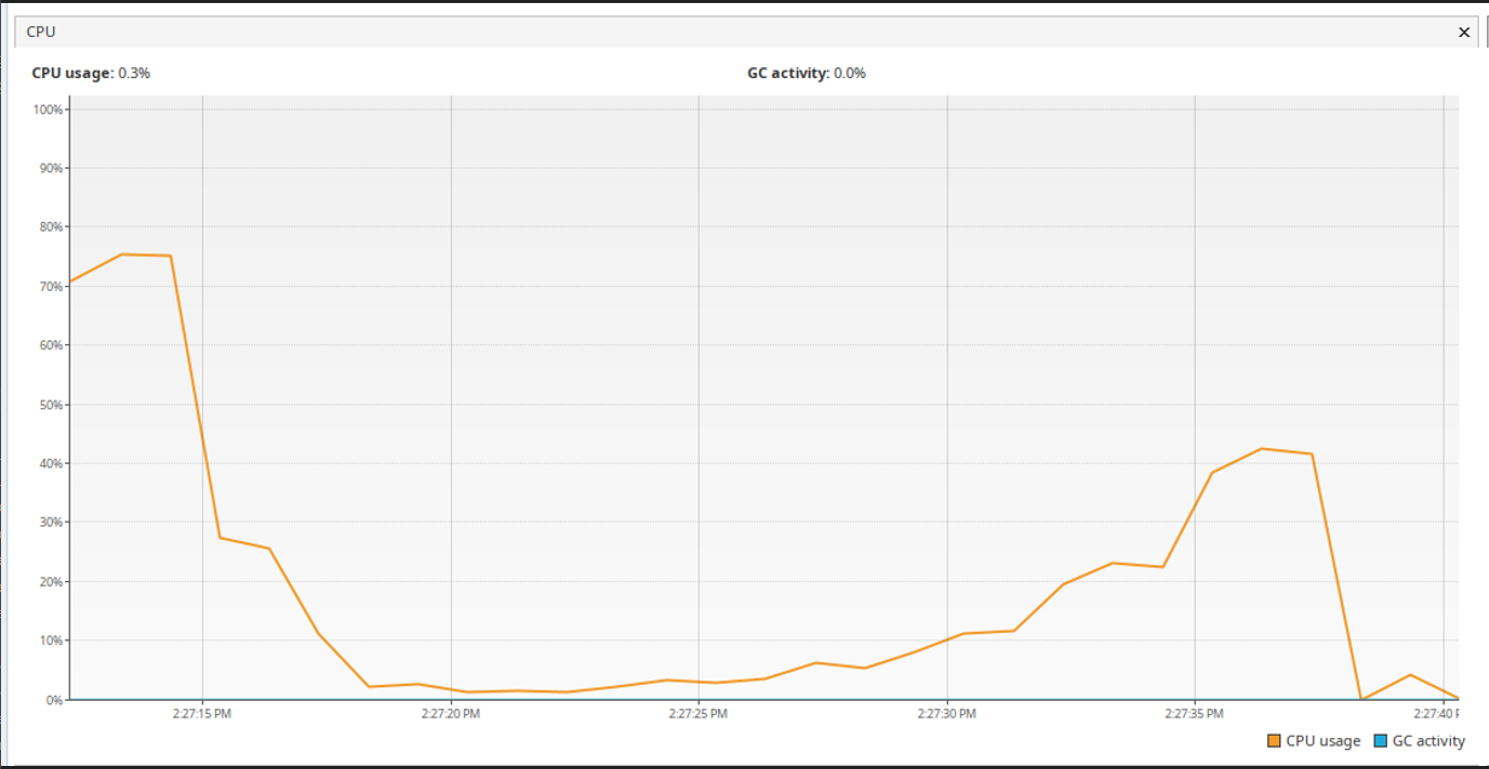
\includegraphics[width=0.8\textwidth]{./Graphs/cpu-susp.png}
     \caption{Benchmark CPU utilization profiling with HtmlFlow-Susp in Spring WebFlux}\label{fig:cpu-susp}
\end{figure}

\begin{figure}[h]
     \centering
     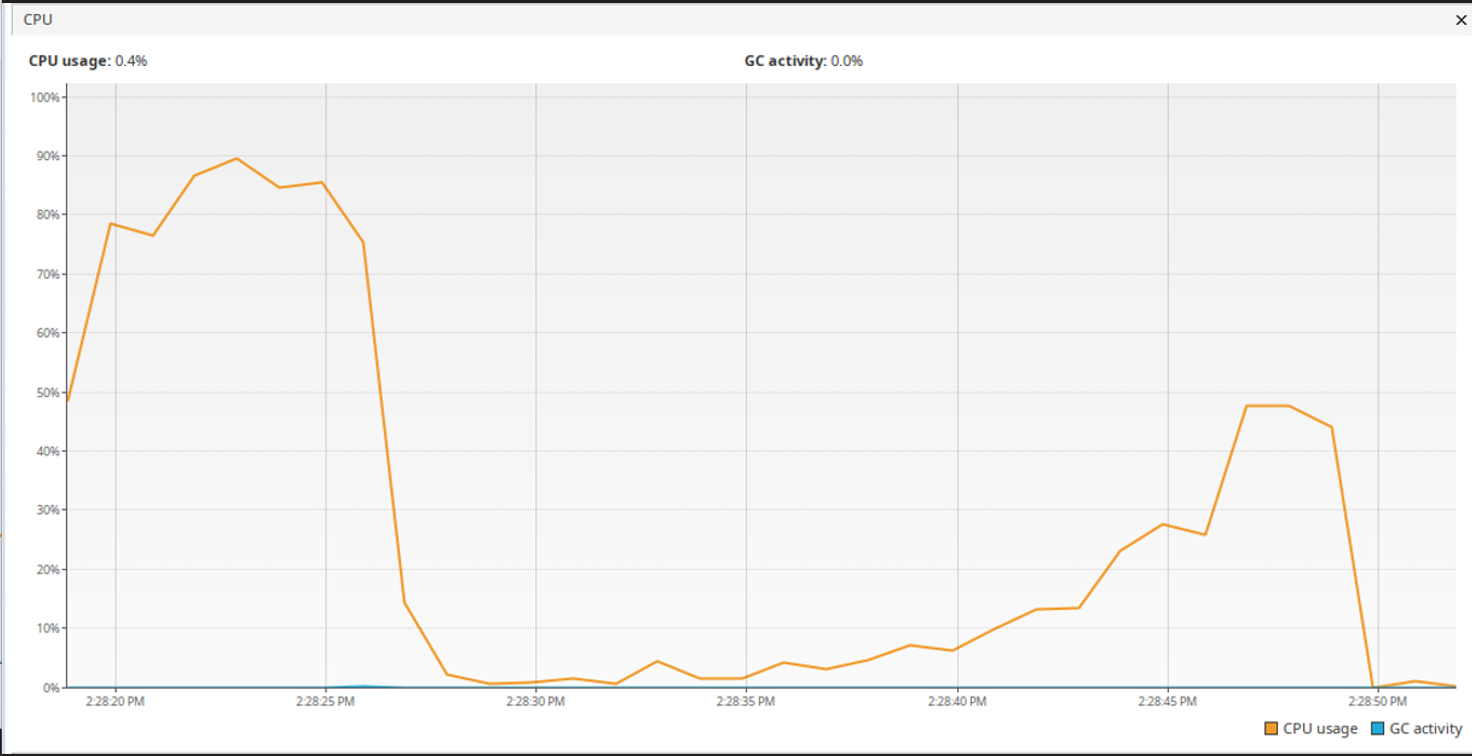
\includegraphics[width=0.8\textwidth]{./Graphs/cpu-virt.png}
     \caption{Benchmark CPU utilization profiling with HtmlFlow running on Virtual Threads in Spring WebFlux}\label{fig:cpu-virt}
\end{figure}

Figures~\ref{fig:cpu-virt} and~\ref{fig:cpu-susp} show CPU utilization profiles
for the \texttt{HtmlFlow-Virtual} and \texttt{HtmlFlow-Susp} implementations,
respectively. \texttt{HtmlFlow-Virtual} reaches peak CPU usage of around 90\%
during load, with sharp transitions between idle and active phases. In
contrast, \texttt{HtmlFlow-Susp} peaks at approximately 75\% and exhibits
smoother transitions, suggesting more efficient CPU scheduling and lower
contention.

\begin{figure}[h]
     \centering
     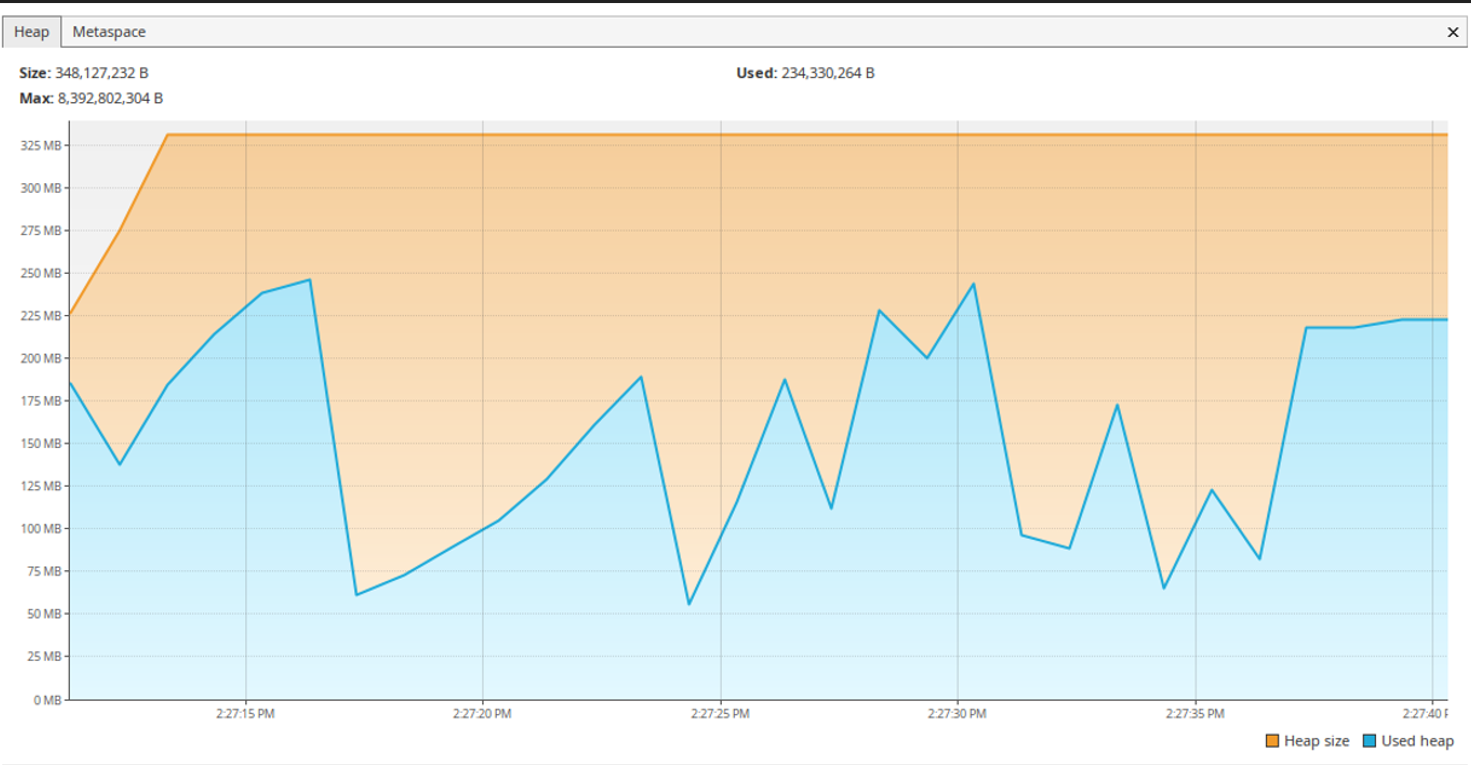
\includegraphics[width=0.8\textwidth]{./Graphs/gc-susp.png}
     \caption{Benchmark memory utilization profiling with HtmlFlow-Susp in Spring WebFlux}\label{fig:gc-susp}
\end{figure}

\begin{figure}[h]
     \centering
     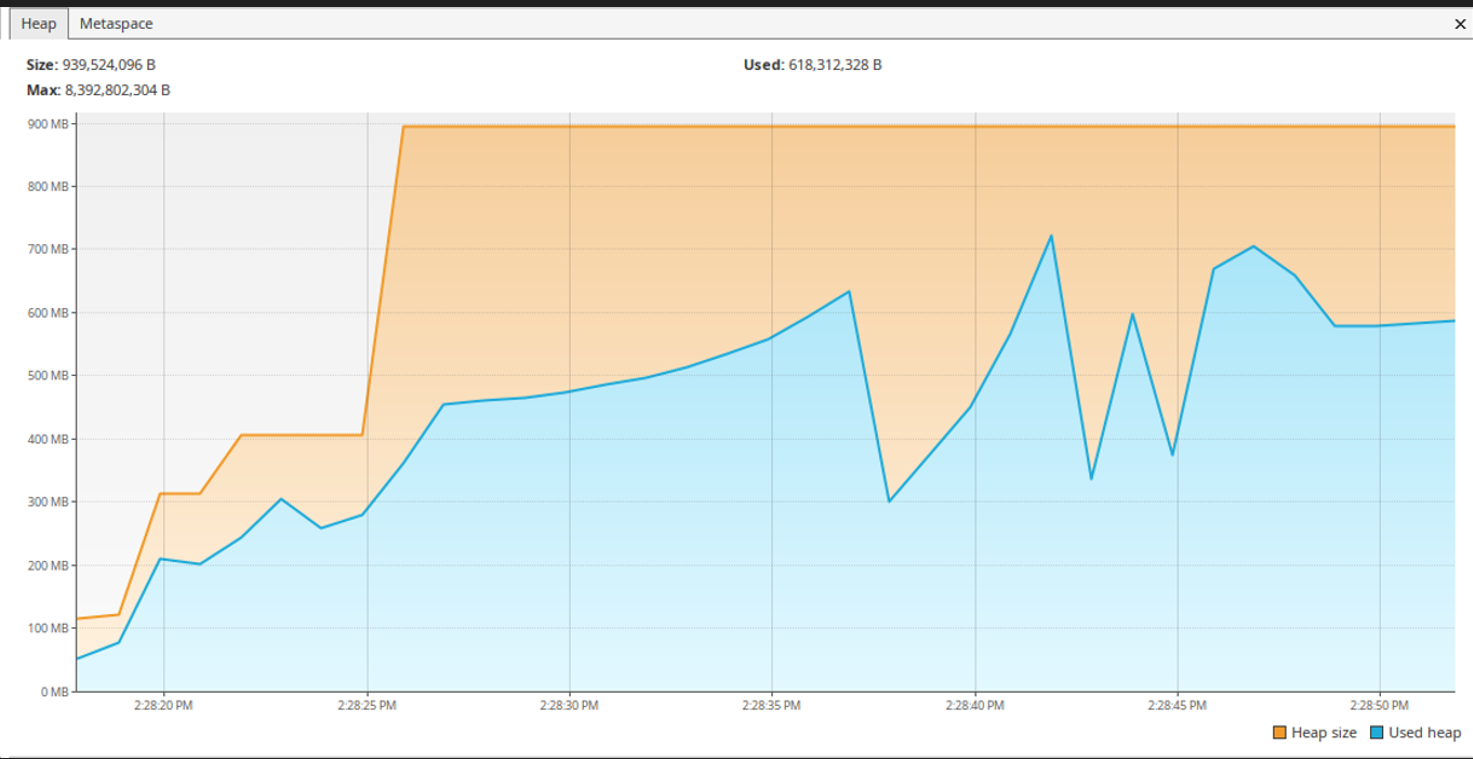
\includegraphics[width=0.8\textwidth]{./Graphs/gc-virt.png}
     \caption{Benchmark memory utilization profiling with HtmlFlow running on Virtual Threads in Spring WebFlux}\label{fig:gc-virt}
\end{figure}

The memory usage disparity is even more pronounced. As shown in
Figure~\ref{fig:gc-virt}, the Virtual Threads implementation gradually climbs
to a peak heap usage of 900MB, with large but infrequent garbage collection
events. Figure~\ref{fig:gc-susp} shows the suspendable version peaks at only
245MB, following a regular sawtooth pattern of small, frequent garbage
collections. Overall, \texttt{HtmlFlow-Virtual} allocates a total of 939MB heap
compared to just 348MB in \texttt{HtmlFlow-Susp}—a 2.7× difference.

\textbf{RxJava Blocking vs Structured Concurrency}

To further assess the efficiency of blocking versus structured concurrency, we
compared the memory behavior of RxJava's \texttt{BlockingObservableIterable}
with \texttt{PublisherAsFlow}. The blocking iterator internally relies on a
lock-based condition variable and an unbounded queue
(\texttt{SpscLinkedArrayQueue}), blocking the thread when no elements are
available. Under high concurrency, this model tends to retain large numbers of
elements in memory, especially when producers outpace consumers. This was
reflected in our profiling, where heap usage for blocking consumption showed
linear growth and irregular GC behavior.

In contrast, \texttt{PublisherAsFlow} employs coroutine-based suspension with
bounded \texttt{Channel} capacity and configurable \texttt{BufferOverflow}
strategies. It requests upstream data based on demand, leveraging structured
concurrency and cooperative cancellation.

It is important to note that our benchmark keeps data items in memory as static
objects, which represents a best-case scenario for memory allocation patterns.
In real-world applications, data typically comes from external sources such as
databases, web services, or file systems, requiring dynamic object creation and
serialization for each request. This would result in significantly higher
memory allocation rates and more frequent garbage collection cycles across all
concurrency models, with the observed differences between Virtual Threads and
suspendable coroutines likely becoming even more pronounced under such
realistic I/O-intensive workloads. While our benchmark demonstrates that
Virtual Threads can achieve comparable throughput to suspendable coroutines, or
other non-blocking paradigms, future work should further explore the impact of
dynamic data sources on memory allocation patterns and garbage collection
behavior to better understand the trade-offs between these concurrency models
in real-world scenarios.

\textbf{Summary of Trade-offs}

While the approaches can achieve similar throughput under load, they differ
significantly in runtime efficiency. Virtual Threads, despite offering a
simplified synchronous style, incur the highest memory and CPU overhead.
structured concurrency delivers superior resource efficiency but
requires familiarity with asynchronous programming constructs. The RxJava
blocking iterator, while easier to adopt in traditional reactive settings,
performs worse in memory-constrained environments due to its unbounded internal
queuing model.

These results suggest that system resource constraints and predictability
requirements should inform the choice of concurrency model. In environments
where memory and CPU resources are limited, structured concurrency via
suspendable coroutines is the most efficient and robust option.